\documentclass{article}
\usepackage[utf8]{inputenc}          % Italian accents
\usepackage[english]{babel}
\usepackage{graphicx}    
\usepackage{amsmath}                 
\usepackage{amsfonts}                
\usepackage{amssymb}    
% extra math symbols             
\usepackage{mathrsfs}                 
\usepackage{bm}
\usepackage{color}
\usepackage[font={small,it},labelfont=bf]{caption} % differentiate captions from normal text
\definecolor{mygreen}{rgb}{0,0.6,0}
\definecolor{mygray}{rgb}{0.5,0.5,0.5}
\definecolor{mymauve}{rgb}{0.58,0,0.82}
\definecolor{Burgundy}{RGB}{144,0,32}
\definecolor{plum}{rgb}{0.56, 0.27, 0.52}
\definecolor{pinegreen}{rgb}{0.0, 0.47, 0.44}
% for including source code snippet
\usepackage{listings}
\usepackage{hyperref} %for using autoref
\usepackage{placeins}

\lstset{ 
	backgroundcolor=\color{white},   % choose the background color; you must add \usepackage{color} or \usepackage{xcolor}; should come as last argument
	basicstyle=\scriptsize,          % the size of the fonts that are used for the code \scriptsize
	breakatwhitespace=false,         % sets if automatic breaks should only happen at whitespace
	breaklines=true,                 % sets automatic line breaking
	captionpos=b,                    % sets the caption-position to bottom
	commentstyle=\color{mygreen},    % comment style
	deletekeywords={...},            % if you want to delete keywords from the given language
	escapeinside={\%*}{*)},          % if you want to add LaTeX within your code
	extendedchars=true,              % lets you use non-ASCII characters; for 8-bits encodings only, does not work with UTF-8
	float=htpb,                        % floating behaviour  
	frame=single,                    % adds a frame around the code
	keepspaces=true,                 % keeps spaces in text, useful for keeping indentation of code (possibly needs columns=flexible)
	keywordstyle=\color{blue},       % keyword style
	language=C++,                	 % the language of the code
	morekeywords={*,...},            % if you want to add more keywords to the set
	numbers=left,                    % where to put the line-numbers; possible values are (none, left, right)
	numbersep=5pt,                   % how far the line-numbers are from the code
	numberstyle=\tiny\color{mygray}, % the style that is used for the line-numbers
	rulecolor=\color{black},         % if not set, the frame-color may be changed on line-breaks within not-black text (e.g. comments (green here))
	showspaces=false,                % show spaces everywhere adding particular underscores; it overrides 'showstringspaces'
	showstringspaces=false,          % underline spaces within strings only
	showtabs=false,                  % show tabs within strings adding particular underscores
	stepnumber=2,                    % the step between two line-numbers. If it's 1, each line will be numbered
	stringstyle=\color{mymauve},     % string literal style
	tabsize=2,                       % sets default tabsize to 2 spaces
	title=\lstname                   % show the filename of files included with \lstinputlisting; also try caption instead of title
}

\begin{document} 
	
	\author{Cesare Cozza \\ Prisco Lo Chiatto }
	\title{Numerical simulation of the longitudinal dispersion bands of phonons in a $(GaAs)_1/(AlAs)_1$ superlattice}
	\maketitle
    
    
\section{Abstract}
A simple linear chain model is used to employ a numerical simulation of the vibrational properties of an ultra-thin $(GaAs)_1/(AlAs)_1$ superlattice. Along the [001] direction, longitudinal Phononic bands are calculated, along with displacements in $\Gamma$ and $GaAs/AlAs$-like LO modes, both in the nearest neighbour and in the next-nearest neighbour approximations.\\
This work shows how even simple models are able to capture the essential features of the physical problems, such as correctly hinting at the presence of confined modes.


    \newpage
\section{Introduction}
\begin{figure}
	\centering
	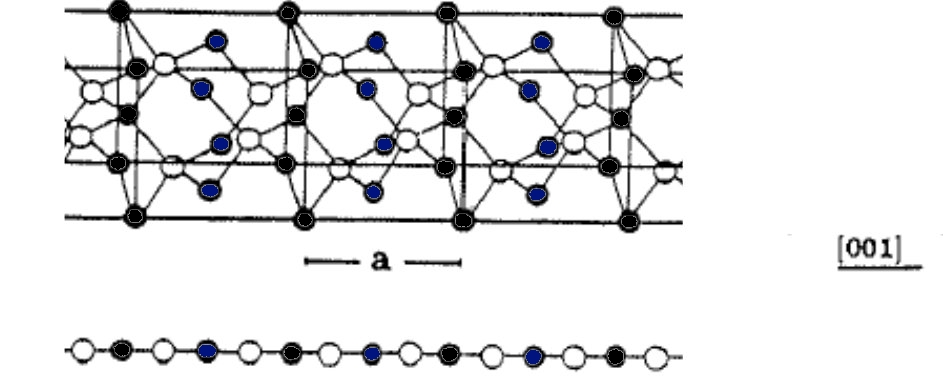
\includegraphics[scale=0.3]{reticolo.jpg}
	\caption{The superlattice used in this study and its projection on the [001] direction. Gallium atoms are painted black, Aluminium ones are blue and Arsenic is white. Note that, when projecting on the [001] direction, each of the planes can be treated as a single atom.}
	\label{fig:reticolo}
\end{figure}

The aim of this work is to study the vibrational properties of a superlattice in a particularly simplified model, to show how even simple models lead to a rather good level of agreement with both more sophisticated theoretical models and experiments.\\
Normal vibrational modes of a quantized elastic system are called phonon. They are collective excitation - i.e. bosonic quasiparticles - and their dispersion relation are related to a number of properties of the system itself. \\
A superlattice is a kind of metamaterial made up from two (or more) materials, in a periodic structure. An ideal $(GaAs)_1/(AlAs)_1$ superlattice is made up from one layer of $GaAs$ followed by one of $AlAs$ in a periodic matter (see \autoref{fig:reticolo}).\smallskip

In general, the vibrational properties of a crystalline solid can be studied through lattice dynamics; thanks to the periodicity of the system the problem can be further reduced to the solution of the dynamics of the atoms in the unitary cell.\\
	Three more approximations will be employed:
	\begin{enumerate}
		\item \textbf{The harmonic approximation}, which consider the atomic cores as simple harmonic oscillator.
		\item \textbf{The nearest neighbour approximation}, where for each atom the interaction between anything other than the closest atoms next to it are neglected.
		\item \textbf{The Born-Oppenheimer approximation}, where ionic and electronic motions can be treated independently.
	\end{enumerate}
	The second will later be relaxed to include also the next to nearest neighbour.\\
	Thanks to these approximation it is possible to reduce the quanto-mechanical problem of vibrations in a solid to the classical one of finding the normal modes. The dispersion bands (how the frequency depends on $\vec{q}$, the wavevector of the mode) can then be found trough a simple numerical algorithm.\\
Only the [0,0,1] direction will be considered, so that the materials' layers follow each other orthogonally with respect to this direction. Only longitudinal vibrations have been taken into account. \\

	\section{Physical Problem}

\begin{figure}
	\centering
	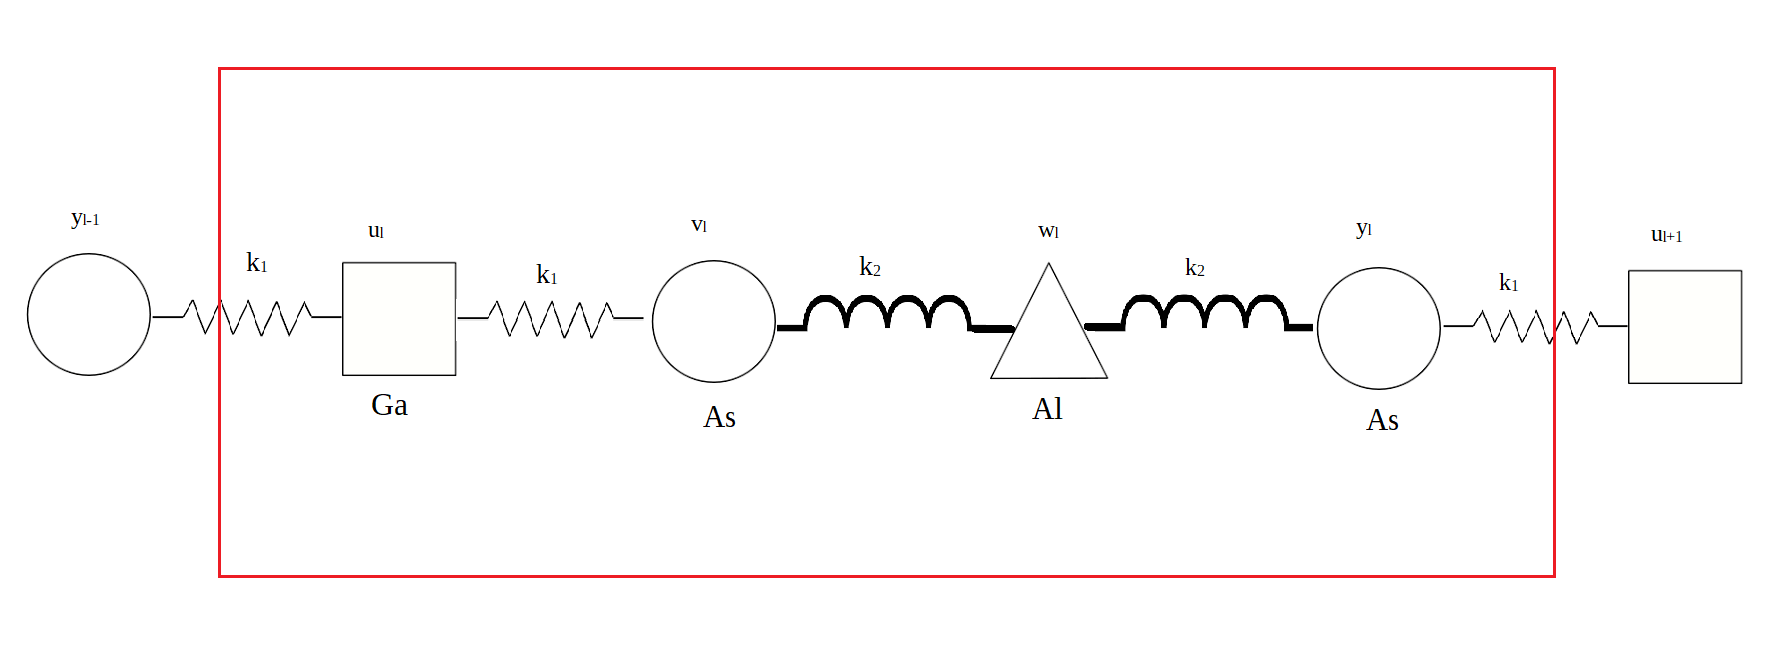
\includegraphics[width=0.7\linewidth]{cella.png}
	\caption{The 4-atom unitary cell analysed in this work in the nearest neighbours approximation.\\
	$k_1$ is the elastic constant between $Ga$ and $As$ and $k_2$ is the elastic constant between $Al$ and $As$. Considering an infinite linear chain $u_l$ represent the displacement of the l-th (arbitrary origin) atom of $Ga$, $v_l$ the displacement of the l-th atom of $As$ of the GaAs molecule, $w_l$ the displacement of the l-th atom of $Al$, $y_l$ the displacement of the l-th atom of $As$ of the $AlAs$ molecule.   }
	\label{fig:cella}
\end{figure}

Because of the approximation used in this study, the relevant physical model is a linear chain of atoms in which the unit cell is made up by 4 atoms, $Ga$-$As$-$Al$-$As$ as in \autoref{fig:cella}, and - at least in first approximation - only interaction with nearest neighbour needs to be taken into account. \\
The following system results (see \autoref{fig:cella} for the meaning of each symbol):
\begin{equation}
	\begin{cases}
	M_{Ga}\ddot{u_l} = -k_1(u_l-v_l) - k_1(u_l-y_{l-1}) \\
	M_{As}\ddot{v_l} = -k_1(v_l-u_l) - k_2(v_l-w_l) \\
	M_{Al}\ddot{w_l} = -k_2(w_l-v_l) - k_2(w_l-y_l) \\
	M_{As}\ddot{y_l} = -k_2(y_l-w_l) - k_1(y_l-u_{l+1}) \\
	\end{cases}
	\label{eq:sistema}	
\end{equation}
To solve this system we impose that every displacement has the form of a plane wave:
\begin{equation}
	\begin{cases}
	u_l = Ue^{i(qla-\omega t)} \\
	v_l = Ve^{i(qla-\omega t)} \\
	w_l = We^{i(qla-\omega t)} \\
	y_l = Ye^{i(qla-\omega t)} \\
	\end{cases}
	\label{eq:onde piane}
\end{equation}
where $a$ is the lattice parameter of the superlattice (sum of the lengths of the respective unit cells).
Solving the system for $\omega$ and then varying $\vec{q}$ will lead to the dispersion bands; since the unit cell has 4 atoms the system to solve is 4-dimensional and so 4 dispersion bands are expected. \par


Similarly, one can obtain the following system when in the next-nearest neighbour approximation (see \autoref{fig:cella2}):

\begin{figure}
	\centering
	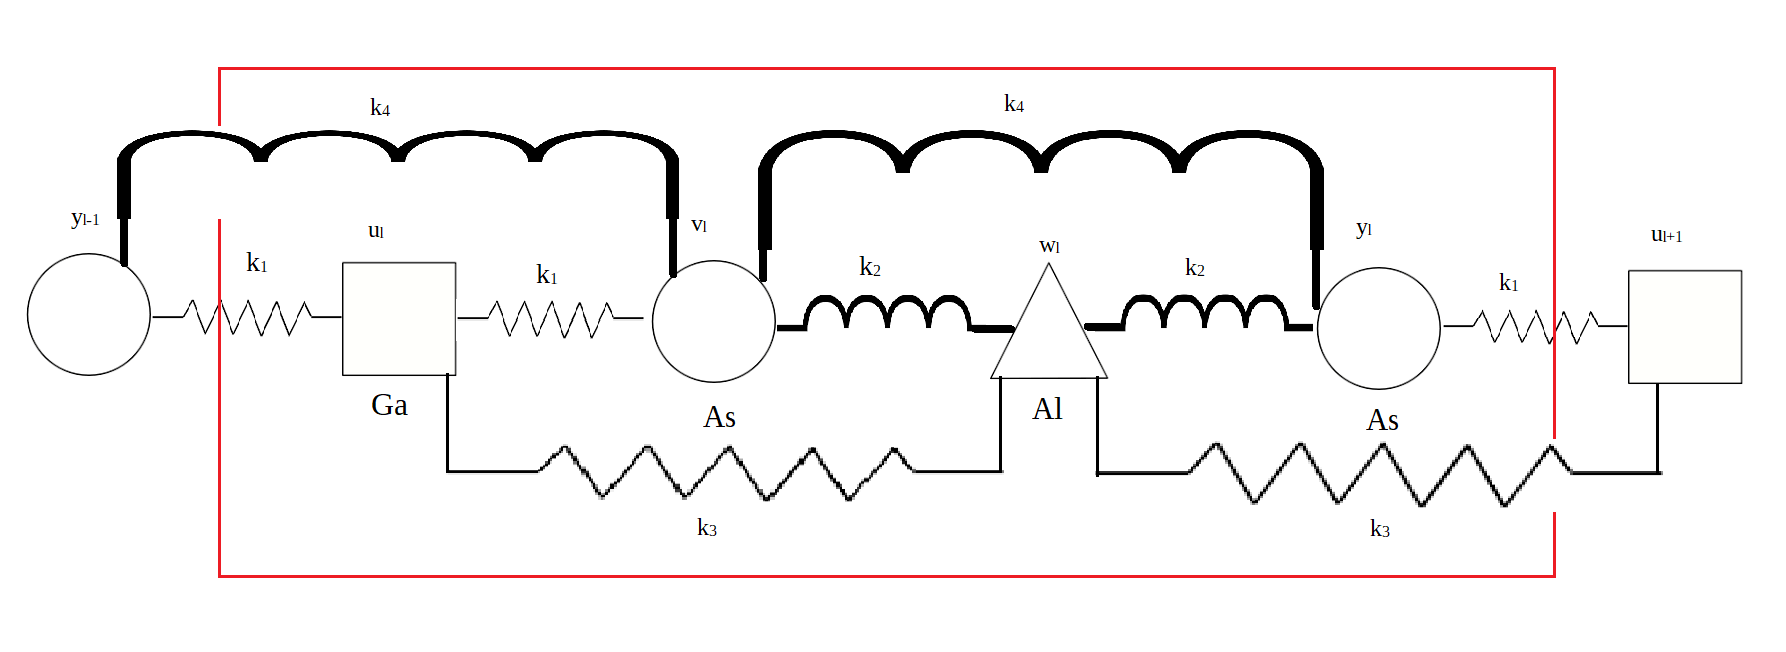
\includegraphics[width=0.7\linewidth]{cella2.png}
	\caption{The 4-atom unitary cell analysed in this work in the next-nearest neighbours approximation.\\
	$k_1$ is the elastic constant between $Ga$ and $As$ and $k_2$ is the elastic constant between $Al$ and $As$, while $k_3$ and $k_4$ are the cation-cation and anion-anion force constants, respectively. Considering an infinite linear chain $u_l$ represent the displacement of the l-th (arbitrary origin) atom of $Ga$, $v_l$ the displacement of the l-th atom of $As$ of the GaAs molecule, $w_l$ the displacement of the l-th atom of $Al$, $y_l$ the displacement of the l-th atom of $As$ of the $AlAs$ molecule.   }
	\label{fig:cella2}
\end{figure}
\begin{equation}
	\begin{cases}
		M_{Ga}\ddot{u_l} = -k_1(u_l-v_l) - k_1(u_l-y_{l-1}) - k_3(u_l -w_{l-1}) - k_3(u_l - w_{l})	 \\
		M_{As}\ddot{v_l} = -k_1(v_l-u_l) - k_2(v_l-w_l)	- k_4(v_l -y_{l-1}) - k_4(v_l - y_{l})	 	 \\
		M_{Al}\ddot{w_l} = -k_2(w_l-v_l) - k_2(w_l-y_l)	- k_3(w_l - u_l) - k_3(w_l - u_{l+1})	 	 \\
		M_{As}\ddot{y_l} = -k_2(y_l-w_l) - k_1(y_l-u_{l+1})- k_4(y_l -v_l) - k_4(y_l - v_{l+1})	  \\
	\end{cases}
	\label{eq:sistema}	
\end{equation}

Values of the force constants are taken from \emph{ab initio} calculations \cite[Table 2]{Molinari}, assuming that they are the same as the single lattice case. Masses, on the other hand, are taken from \cite{IUPAC}.
Since the force constant $k_1$ and $k_2$ are so similar (equal up to less than 5\%), their difference can be neglected, substituting to both of them their average value. This is sometimes called the “Mass approximation”, since only the mass difference between the two atoms is taken into account. Of course, neglecting also the mass difference would take the problem back to a simple lattice instead of a superlattice.\\
As for the next-nearest neighbour case, $k_3$($k_4$) is taken to be the average of the anion-anion(cation-cation) constant of $GaAs$ and $AlAs$.

\newpage
\section{Numerical solution}
The problem of finding the dispersion bands of GaAs/AlAs reduces - in the nearest neighbour approximation - to the solution of the system showed in \autoref{eq:sistema}. \\
Substituting into the system the solution for the plain wave in \autoref{eq:onde piane}, after some algebra one gets:
\begin{equation}
	\begin{cases}
		(-\omega^2M_{Ga} + 2k_1)U - k_1V - (k_1e^{-iqa})Y = 0 \\
		-k_1U -k_2W + (-\omega^2M_{As} + k_1 + k_2)V = 0 \\
		(-\omega^2M_{Al} + 2k_2)W -k_2V - k_2Y = 0 \\
		-(k_1e^{iqa})U - k_2W + (-\omega^2M_{As} + k_1 + k_2)Y = 0	
	\end{cases}
	\label{sist.final}
\end {equation}

This is convenient as the system's associated matrix is already written in the form $[-\omega^2I + A]$, where
\begin{equation} 
A = \begin{pmatrix}
   \frac{2k_1}{M_{Ga}}				& -\frac{k_1}{M_{Ga}}  			 & 0  			 & -\frac{k_1}{M_{Ga}}e^{-iqa}  \\ 
   -\frac{k_1}{M_{As}} 				& \frac{k_1}{M_{As}}+\frac{k_2}{M_{As}}  & -\frac{k_2}{M_{As}}    & 0  \\ 
   0						& -\frac{k_2}{M_{Al}}  			 & \frac{2k_2}{M_{Al}} 	 & -\frac{k_2}{M_{Al}}  \\ 
   -\frac{k_1}{M_{As}}e^{iqa} 			& 0 					 & -\frac{k_2}{M_{As}}    & \frac{k_1}{M_{As}}+\frac{k_2}{M_{As}}   
\end{pmatrix} 
\label{eq:matrice}
\end{equation}


so it is possible to solve the secular equation and find $\omega^2$. Varying $q$ inside the first Brillouin Zone (the direction is fixed so only the magnitude varies) one arrives at the dispersion relation, whereas the eigenvectors of A are the displacement of the single atoms in the chain.\par
Similarly, for next-nearest neighbour:

\begin{equation} 
A' = \begin{pmatrix}
	\frac{2(k_1+k_3)}{M_{Ga}}				& -\frac{k_1}{M_{Ga}}  			 & -\frac{k_3(1+e^{-iqa})}{M_{Ga}} & -\frac{k_1}{M_{Ga}}e^{-iqa}  \\ 
		-\frac{k_1}{M_{As}} 						& \frac{k_1+k_2+2k_4}{M_{As}} 				 & -\frac{k_2}{M_{As}}             & -\frac{k_4(1+e^{-iqa})}{M_{As}}\\ 
		\frac{k_3(1+e^{iqa})}{M_{Al}}				& -\frac{k_2}{M_{Al}}  		 	& \frac{2(k_2+k_3)}{M_{Al}} 	 & -\frac{k_2}{M_{Al}}  \\ 
	 -\frac{k_1}{M_{As}}e^{iqa} 			& -\frac{k_4(1+e^{iqa})}{M_{As}} 					 & -\frac{k_2}{M_{As}}    & \frac{k_1+k_2+2k_4}{M_{As}}   
\end{pmatrix} 
\label{eq:matrice}
\end{equation}

\medskip

To obtain the solution of the problem a numerical approach was undertaken: a program in C++ has been written which, after discretising the Brillouin Zone in a selected number of points, calculates the appropriate wavevector $q$ for each points, and then fills the matrix in \autoref{eq:matrice} with the appropriate values. Finally, using a subroutine of the $Eigen$ linear algebra package, it finds eigenvectors and eigenvalues for each matrix.\\
The result is a discretized version of the dispersion relation, which is then plotted using GNUPLOT. \par
To check that the eigenvectors and eigenvalues are self-consistent, the following quantity is calculated:
\begin{equation}
max_{i}(\frac{A*v_{i} - \lambda_i*v_i}{\lambda_i*v_i})
	\label{<+label+>}
\end{equation}
where $v_i$ is the i-th eigenvector as calculated by the subroutine and $\lambda_i$ its corresponding eigenvalues. Values near machine-eps are expected.

\section{Results and Comparison} 
\begin{figure}[ht]
	\centering
	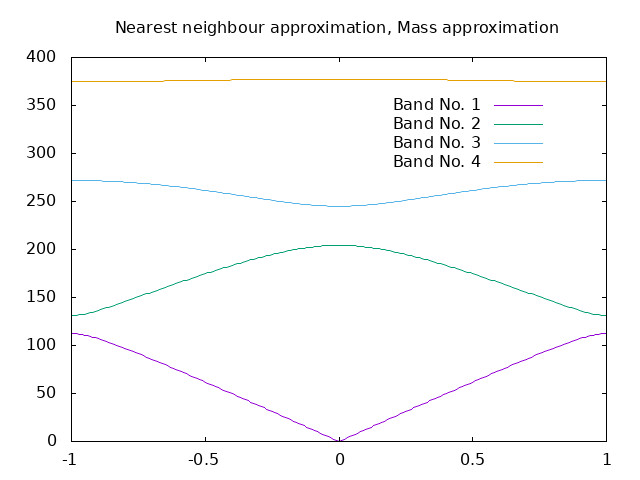
\includegraphics[scale=0.3]{same.jpeg}
	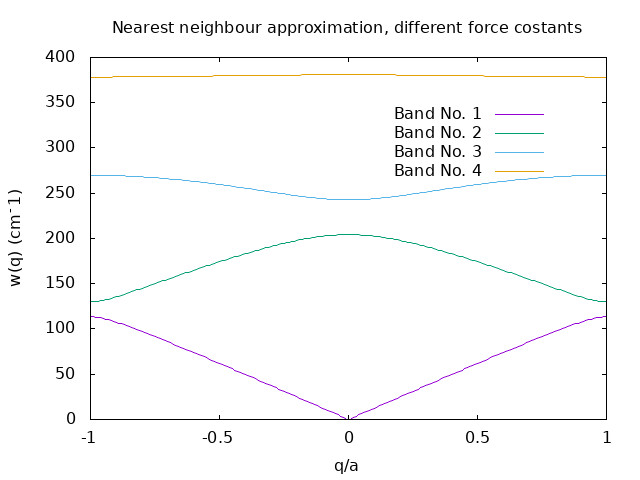
\includegraphics[scale=0.3]{different.jpeg}
	\caption{Calculated band structure in the [001] direction.\\ \textbf{Left:} using nearest neighbour and Mass approximations. \textbf{Right:} using only nearest neighbour approximation. It's evident how similar the two results are, justifying the Mass approximation.\\
	Band 3 and 4 are those that give rise to $GaAs$ and $AlAs$-like LO modes, respectively.}
	\label{fig:nearest}
\end{figure}
\begin{figure}[ht]
	\centering
	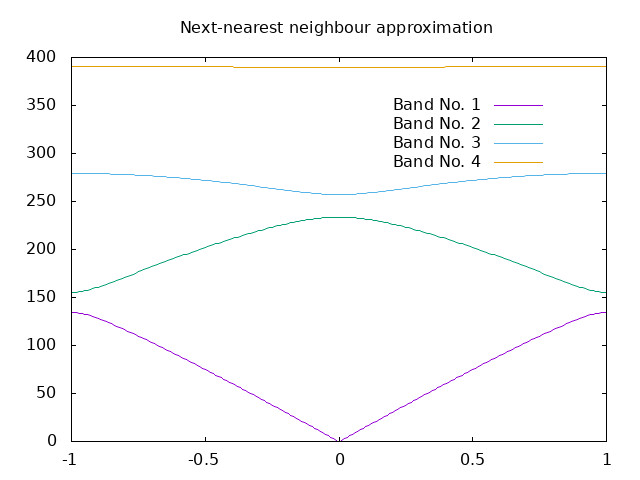
\includegraphics[scale=0.3]{second.jpeg}
	\caption{Calculated band structure in the [001] direction, using next-nearest neighbour approximations. It appears as an upward shifted version of the nearest neighbour one, but also features reduced band-gaps.}
	\label{fig:second}
\end{figure}
In \autoref{fig:nearest} one can see the band structure as calculated using the Mass and nearest neighbours approximations, only the nearest neighbours approximation, while the results of the next-nearest neighbour approximation is shown in \autoref{fig:second}. \autoref{fig:ampiezze} shows the amplitude of the normal modes in $\Gamma$.\par
\begin{figure}[hp]
	\centering
	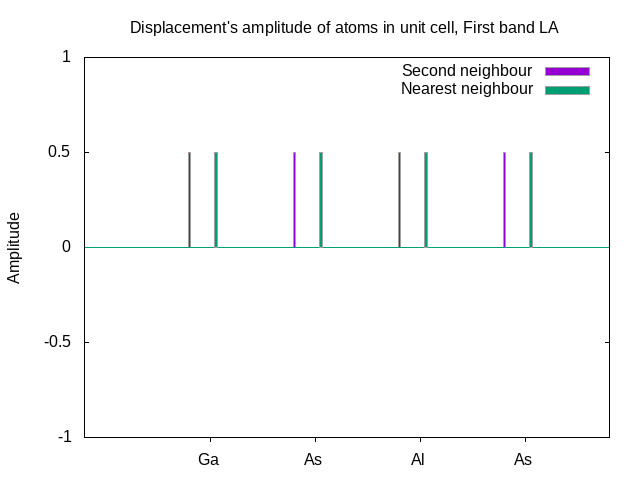
\includegraphics[scale=0.35]{ampiezze1.jpg}
	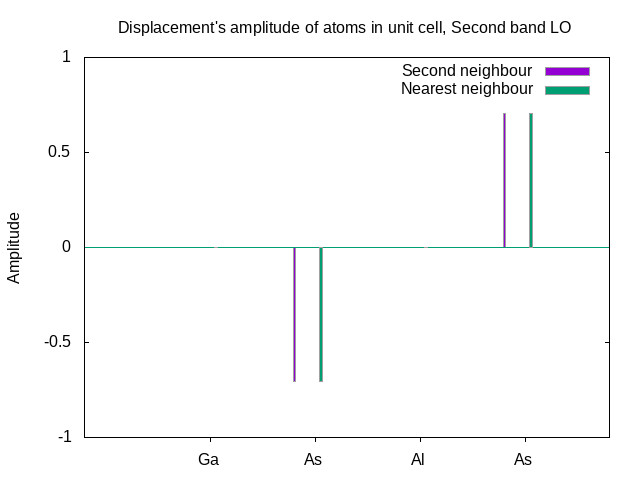
\includegraphics[scale=0.35]{ampiezze2.jpg}
	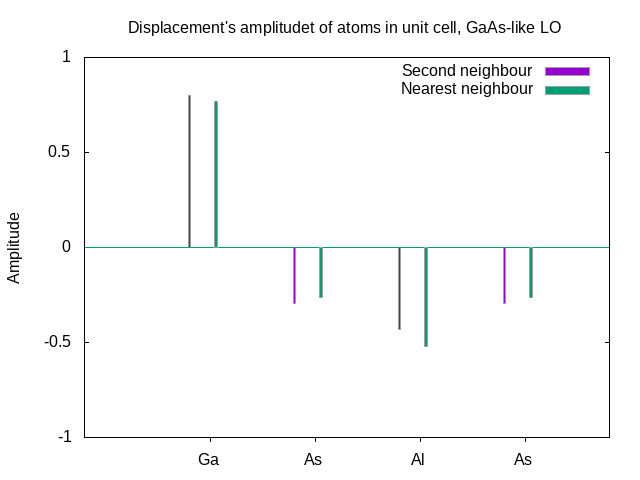
\includegraphics[scale=0.35]{ampiezze3.jpg}
	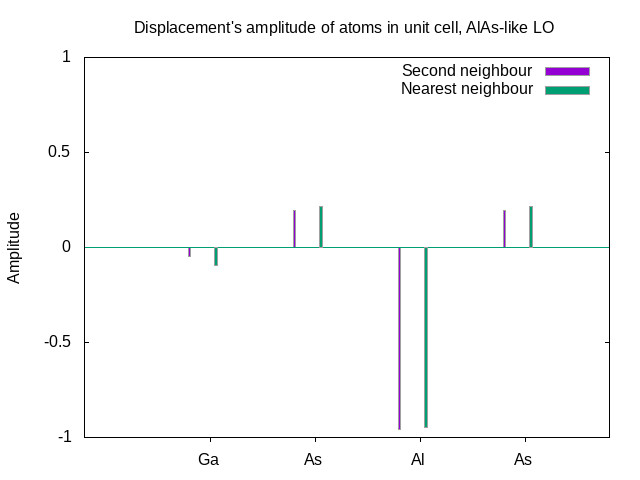
\includegraphics[scale=0.35]{ampiezze4.jpg}
	\caption{Calculated amplitudes ({\color{pinegreen} nearest neighbour} and {\color{plum} next-nearest neighbour})  of the four bands, in the high symmetry point $\Gamma$.\\ The first mode appropriately is a rigid translation, since it's a zero frequency mode. The third and fourth mode should respectively be the $GaAs$-like and $AlAs$-like LO modes. While the $AlAs$-like modes does indeed display some degree of confinement, no such thing can be said for the $GaAs$-like mode, showing the limitation of this simple model.}
	\label{fig:ampiezze}
\end{figure}
The results whose comparison to known literature is easier is the frequency of the $GaAs$($AlAs$)-like modes; this is because these frequency can be obtained from Raman spectroscopy and in part because their interpretation had a certain degree of controversy when they were first observed \cite{Molinari}. Direct comparison with (\cite[Fig.6]{Molinari},\cite{Cardona}) can be done, to see how the present works stacks up with theoretical (from linear response DFT)  and experimental values found in literature. Comparison can be seen in \autoref{tab:frequenze}.\\
\medskip

\begin{table}
	\centering
	\begin{tabular}{||l|c|c|c|c||}
		\hline
		& Present Work (NN) & Present Work (SN)& Theory \cite{Molinari} & Experiment \cite{Cardona} \\
			\hline
		GaAs-like & 245 &257 &266&275 \\
		\hline
		AsAl-like & 377 & 389&399&385 \\
		\hline
	\end{tabular}
	\caption{Comparison of LO modes frequency. The first two columns are values calculated in the present work, with Nearest-Neighbour (NN) and Next-Nearest Neighbour approximation, then the values calculated in \cite{Molinari} using DFT and values obtained from Raman spectroscopy in \cite{Cardona}.\\
	All values in $cm^{-1}$.}
	\label{tab:frequenze}
\end{table}

\newpage
\section{Conclusions}
A simple model has been used to calculate the vibrational properties of an “ultra-thin” $GaAs$/$AlAs$ as a linear chain of atoms oscillating along the [001] direction.\\
Comparison of the $GaAs$/$AlAs$-like frequencies to both experiment and more sophisticated theoretical models gives a satisfactory level of agreement, given the crudeness of the model. On the other hand, confinement is only partially exhibited by this model, as show by looking at the amplitudes of the normal modes.

\appendix
\newpage
\begin{thebibliography}{9}
	\bibitem{Molinari}
		E.Molinari, S.Baroni, P.Giannozzi, S. de Gironcoli (1991).
		\emph{Phonon spectra of ultrathin $GaAs/AlAs$ superlattices: An} ab initio \emph{calculation.} {\color{Burgundy} Light Scattering in Semiconductor Structures and Superlattices \textbf{(pp 39-52)}}
	\bibitem{IUPAC}
		Juris Meija \emph{et al.} (2016).\emph{"Atomic weights of the elements 2013 (IUPAC Technical Report)".} {\color{Burgundy} Pure Appl. Chem. \textbf{88 (3)}: 265–291.}
	\bibitem{Cardona}
		M.Cardona, T.Suemoto, N.E. Christensen, T.Isu, K.Ploog (1987)
		\emph{Electronic and vibronic structure of the $(GaAs)_1(AlAs)_1$ superlattice.} {\color{Burgundy} PRL B \textbf{36}, 5906}
\end{thebibliography}
\end{document}
